\documentclass{standalone}
\usepackage{tikz}
\usetikzlibrary{patterns, positioning}

\begin{document}
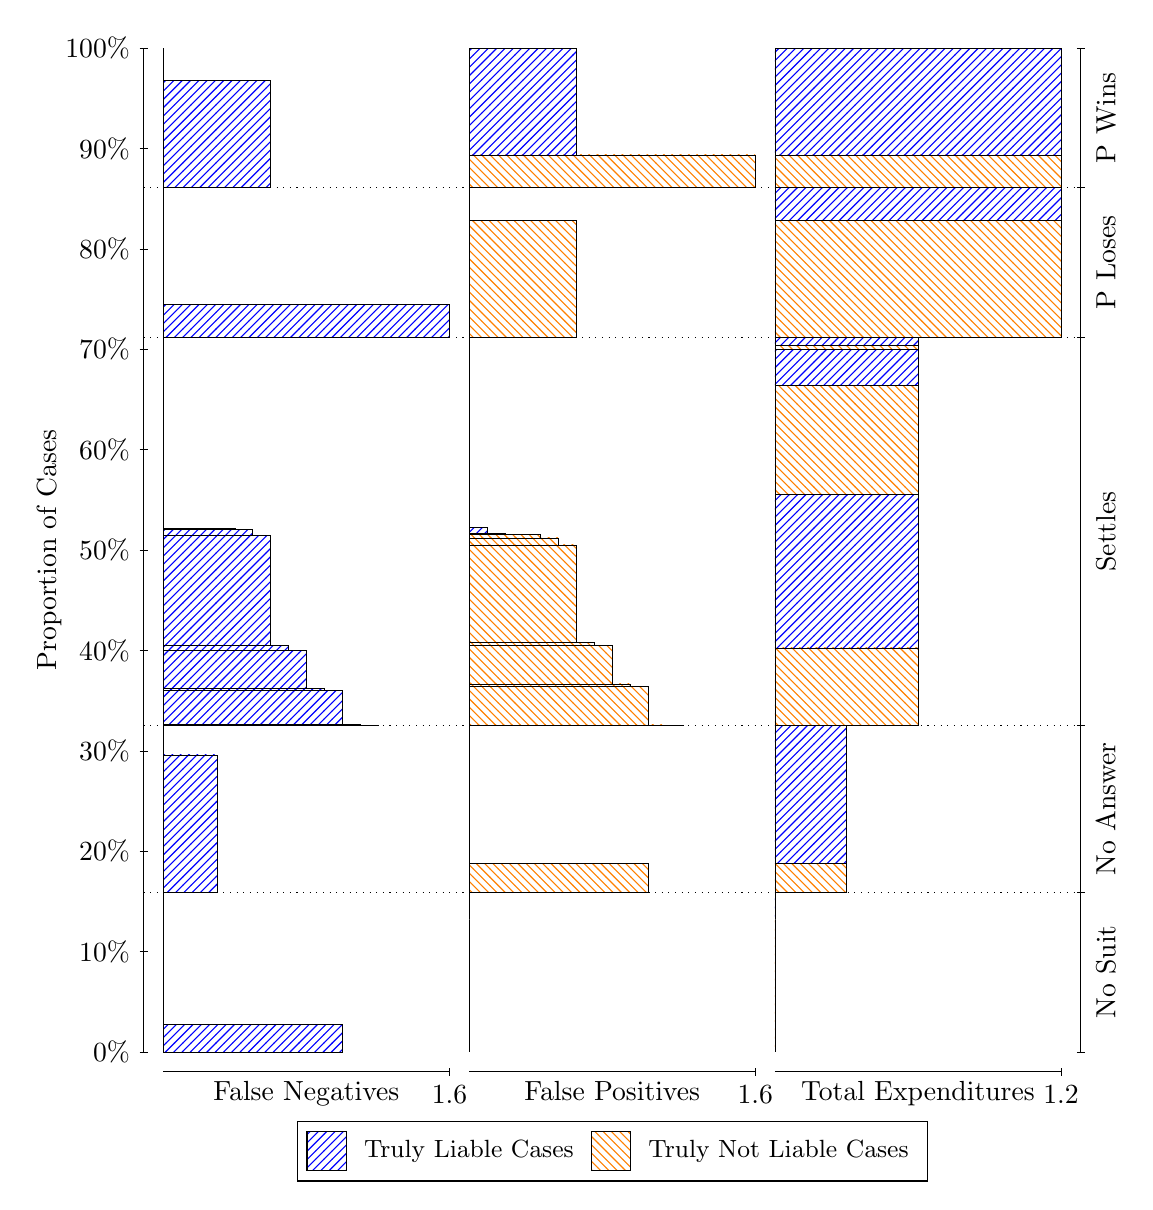
\begin{tikzpicture}
\draw[black, very thin] (1.5,1.75) -- (1.5,14.5);
\node[rotate=90, anchor=center] at (0.3, 8.125) {Proportion of Cases};
\draw[black, very thin] (1.45,1.75) -- (1.55,1.75);
\node[anchor=east] at (1.45, 1.75) {0\%};
\draw[black, very thin] (1.45,3.025) -- (1.55,3.025);
\node[anchor=east] at (1.45, 3.025) {10\%};
\draw[black, very thin] (1.45,4.3) -- (1.55,4.3);
\node[anchor=east] at (1.45, 4.3) {20\%};
\draw[black, very thin] (1.45,5.575) -- (1.55,5.575);
\node[anchor=east] at (1.45, 5.575) {30\%};
\draw[black, very thin] (1.45,6.85) -- (1.55,6.85);
\node[anchor=east] at (1.45, 6.85) {40\%};
\draw[black, very thin] (1.45,8.125) -- (1.55,8.125);
\node[anchor=east] at (1.45, 8.125) {50\%};
\draw[black, very thin] (1.45,9.4) -- (1.55,9.4);
\node[anchor=east] at (1.45, 9.4) {60\%};
\draw[black, very thin] (1.45,10.675) -- (1.55,10.675);
\node[anchor=east] at (1.45, 10.675) {70\%};
\draw[black, very thin] (1.45,11.95) -- (1.55,11.95);
\node[anchor=east] at (1.45, 11.95) {80\%};
\draw[black, very thin] (1.45,13.225) -- (1.55,13.225);
\node[anchor=east] at (1.45, 13.225) {90\%};
\draw[black, very thin] (1.45,14.5) -- (1.55,14.5);
\node[anchor=east] at (1.45, 14.5) {100\%};

\draw[black, very thin] (13.4,1.75) -- (13.4,14.5);
\draw[black, very thin] (13.35,1.75) -- (13.45,1.75);
\node[anchor=west] at (13.35, 1.75) {};
\draw[black, very thin] (13.35,3.7802) -- (13.45,3.7802);
\node[anchor=west] at (13.35, 3.7802) {};
\draw[black, very thin] (13.35,5.8933) -- (13.45,5.8933);
\node[anchor=west] at (13.35, 5.8933) {};
\draw[black, very thin] (13.35,10.828) -- (13.45,10.828);
\node[anchor=west] at (13.35, 10.828) {};
\draw[black, very thin] (13.35,12.727) -- (13.45,12.727);
\node[anchor=west] at (13.35, 12.727) {};
\draw[black, very thin] (13.35,14.5) -- (13.45,14.5);
\node[anchor=west] at (13.35, 14.5) {};

\draw[black, very thin, pattern color=blue, pattern=north east lines] (1.75,1.75) rectangle (4.0208,2.0989);
\draw[black, very thin, pattern color=orange, pattern=north west lines] (1.75,2.0989) rectangle (1.75,3.7802);
\draw[black, very thin, pattern color=blue, pattern=north east lines] (1.75,3.7802) rectangle (2.4312,5.5236);
\draw[black, very thin, pattern color=orange, pattern=north west lines] (1.75,5.5236) rectangle (1.75,5.8933);
\draw[black, very thin, pattern color=blue, pattern=north east lines] (1.75,5.8933) rectangle (4.475,5.8964);
\draw[black, very thin, pattern color=blue, pattern=north east lines] (1.75,5.8964) rectangle (4.2479,5.9057);
\draw[black, very thin, pattern color=blue, pattern=north east lines] (1.75,5.9057) rectangle (4.0208,6.3445);
\draw[black, very thin, pattern color=blue, pattern=north east lines] (1.75,6.3445) rectangle (3.7937,6.349);
\draw[black, very thin, pattern color=blue, pattern=north east lines] (1.75,6.349) rectangle (3.7937,6.3699);
\draw[black, very thin, pattern color=blue, pattern=north east lines] (1.75,6.3699) rectangle (3.5667,6.8518);
\draw[black, very thin, pattern color=blue, pattern=north east lines] (1.75,6.8518) rectangle (3.3396,6.9166);
\draw[black, very thin, pattern color=blue, pattern=north east lines] (1.75,6.9166) rectangle (3.1125,8.3099);
\draw[black, very thin, pattern color=blue, pattern=north east lines] (1.75,8.3099) rectangle (2.8854,8.3819);
\draw[black, very thin, pattern color=blue, pattern=north east lines] (1.75,8.3819) rectangle (2.6583,8.4023);
\draw[black, very thin, pattern color=orange, pattern=north west lines] (1.75,8.4023) rectangle (1.75,10.828);
\draw[black, very thin, pattern color=blue, pattern=north east lines] (1.75,10.828) rectangle (5.3833,11.244);
\draw[black, very thin, pattern color=orange, pattern=north west lines] (1.75,11.244) rectangle (1.75,12.727);
\draw[black, very thin, pattern color=blue, pattern=north east lines] (1.75,12.727) rectangle (3.1125,14.085);
\draw[black, very thin, pattern color=orange, pattern=north west lines] (1.75,14.085) rectangle (1.75,14.5);
\draw[black, very thin, pattern color=orange, pattern=north west lines] (5.6333,1.75) rectangle (5.6333,3.4312);
\draw[black, very thin, pattern color=blue, pattern=north east lines] (5.6333,3.4312) rectangle (5.6333,3.7802);
\draw[black, very thin, pattern color=orange, pattern=north west lines] (5.6333,3.7802) rectangle (7.9042,4.1498);
\draw[black, very thin, pattern color=blue, pattern=north east lines] (5.6333,4.1498) rectangle (5.6333,5.8933);
\draw[black, very thin, pattern color=orange, pattern=north west lines] (5.6333,5.8933) rectangle (8.3583,5.8948);
\draw[black, very thin, pattern color=orange, pattern=north west lines] (5.6333,5.8948) rectangle (8.1313,5.9033);
\draw[black, very thin, pattern color=orange, pattern=north west lines] (5.6333,5.9033) rectangle (7.9042,6.395);
\draw[black, very thin, pattern color=orange, pattern=north west lines] (5.6333,6.395) rectangle (7.6771,6.4245);
\draw[black, very thin, pattern color=orange, pattern=north west lines] (5.6333,6.4245) rectangle (7.45,6.9132);
\draw[black, very thin, pattern color=orange, pattern=north west lines] (5.6333,6.9132) rectangle (7.2229,6.9528);
\draw[black, very thin, pattern color=orange, pattern=north west lines] (5.6333,6.9528) rectangle (6.9958,8.1909);
\draw[black, very thin, pattern color=orange, pattern=north west lines] (5.6333,8.1909) rectangle (6.7687,8.279);
\draw[black, very thin, pattern color=orange, pattern=north west lines] (5.6333,8.279) rectangle (6.5417,8.3192);
\draw[black, very thin, pattern color=blue, pattern=north east lines] (5.6333,8.3192) rectangle (6.0875,8.3397);
\draw[black, very thin, pattern color=blue, pattern=north east lines] (5.6333,8.3397) rectangle (5.8604,8.4116);
\draw[black, very thin, pattern color=blue, pattern=north east lines] (5.6333,8.4116) rectangle (5.6333,10.828);
\draw[black, very thin, pattern color=orange, pattern=north west lines] (5.6333,10.828) rectangle (6.9958,12.312);
\draw[black, very thin, pattern color=blue, pattern=north east lines] (5.6333,12.312) rectangle (5.6333,12.727);
\draw[black, very thin, pattern color=orange, pattern=north west lines] (5.6333,12.727) rectangle (9.2667,13.142);
\draw[black, very thin, pattern color=blue, pattern=north east lines] (5.6333,13.142) rectangle (6.9958,14.5);
\draw[black, very thin, pattern color=orange, pattern=north west lines] (9.5167,1.75) rectangle (9.5167,3.4312);
\draw[black, very thin, pattern color=blue, pattern=north east lines] (9.5167,3.4312) rectangle (9.5167,3.7802);
\draw[black, very thin, pattern color=orange, pattern=north west lines] (9.5167,3.7802) rectangle (10.425,4.1498);
\draw[black, very thin, pattern color=blue, pattern=north east lines] (9.5167,4.1498) rectangle (10.425,5.8933);
\draw[black, very thin, pattern color=orange, pattern=north west lines] (9.5167,5.8933) rectangle (11.333,6.8821);
\draw[black, very thin, pattern color=blue, pattern=north east lines] (9.5167,6.8821) rectangle (11.333,8.8292);
\draw[black, very thin, pattern color=orange, pattern=north west lines] (9.5167,8.8292) rectangle (11.333,10.22);
\draw[black, very thin, pattern color=blue, pattern=north east lines] (9.5167,10.22) rectangle (11.333,10.675);
\draw[black, very thin, pattern color=orange, pattern=north west lines] (9.5167,10.675) rectangle (11.333,10.722);
\draw[black, very thin, pattern color=blue, pattern=north east lines] (9.5167,10.722) rectangle (11.333,10.828);
\draw[black, very thin, pattern color=orange, pattern=north west lines] (9.5167,10.828) rectangle (13.15,12.312);
\draw[black, very thin, pattern color=blue, pattern=north east lines] (9.5167,12.312) rectangle (13.15,12.727);
\draw[black, very thin, pattern color=orange, pattern=north west lines] (9.5167,12.727) rectangle (13.15,13.142);
\draw[black, very thin, pattern color=blue, pattern=north east lines] (9.5167,13.142) rectangle (13.15,14.5);
\draw[black, dotted] (1.5,3.7802) -- (13.4,3.7802);
\draw[black, dotted] (1.5,5.8933) -- (13.4,5.8933);
\draw[black, dotted] (1.5,10.828) -- (13.4,10.828);
\draw[black, dotted] (1.5,12.727) -- (13.4,12.727);
\draw[black, very thin] (1.75,1.5) -- (5.3833,1.5);
\node[anchor=north] at (3.5667, 1.5) {False Negatives};
\draw[black, very thin] (5.3833,1.45) -- (5.3833,1.55);
\node[anchor=north] at (5.3833, 1.45) {1.6};

\draw[black, very thin] (5.6333,1.5) -- (9.2667,1.5);
\node[anchor=north] at (7.45, 1.5) {False Positives};
\draw[black, very thin] (9.2667,1.45) -- (9.2667,1.55);
\node[anchor=north] at (9.2667, 1.45) {1.6};

\draw[black, very thin] (9.5167,1.5) -- (13.15,1.5);
\node[anchor=north] at (11.333, 1.5) {Total Expenditures};
\draw[black, very thin] (13.15,1.45) -- (13.15,1.55);
\node[anchor=north] at (13.15, 1.45) {1.2};

\node[black, centered, rotate=90] at (13.72, 2.7651) {No Suit};
\node[black, centered, rotate=90] at (13.72, 4.8367) {No Answer};
\node[black, centered, rotate=90] at (13.72, 8.3608) {Settles};
\node[black, centered, rotate=90] at (13.72, 11.778) {P Loses};
\node[black, centered, rotate=90] at (13.72, 13.614) {P Wins};

\draw (7.449999999999999,1.5) node[draw=none] (baseCoordinate) {};
\begin{scope}[align=center]
        \matrix[scale=0.5, draw=black, below=0.5cm of baseCoordinate, nodes={draw}, column sep=0.1cm]{
            \node[rectangle, draw, minimum width=0.5cm, minimum height=0.5cm, pattern=north east lines, pattern color=blue] {}; &
            \node[draw=none, font=\small] (B) {Truly Liable Cases}; &
            \node[rectangle, draw, minimum width=0.5cm, minimum height=0.5cm, pattern=north west lines, pattern color=orange] {}; &
            \node[draw=none, font=\small] (B) {Truly Not Liable Cases}; \\
            };
\end{scope}

\end{tikzpicture}
\end{document}